%!TEX root = ../../thesis.tex
%!TEX enableSynctex = true
%*******************************************************************************
%****************************** Third Chapter **********************************
%*******************************************************************************
% **************************** Define Graphics Path **************************
\ifpdf
    \graphicspath{{Chapters/literature/Figs/Raster/}{Chapters/literature/Figs/PDF/}{Chapters/literature/Figs/}}
\else
    \graphicspath{{Chapters/literature/Figs/Vector/}{Chapters/Figs/}}
\fi

% Should include phototoxictiy http://www.nature.com/nmeth/journal/v14/n7/full/nmeth.4344.html

% Words to use: archetypal

\chapter{Contemporary \gls{light-sheet} microscope technology}\label{chapter:literature}

\gls{LSFM} is revolutionising the way in which complex, living biological samples can be imaged at high spatial and temporal resolution. %-
The technique differs from conventional \gls{epi-fluorescence} microscopy in that the sample is illuminated orthogonally to the detection axis as shown in \figurename~\ref{fig:epi_con_lsfm}.
The decoupling of illumination and excitation allows for the construction of light sheets which excite a single plane of interest, which are thin in the direction of the optical axis of the detection system.%~\cite{14,15,16}.
As such, the technique offers \gls{optical sectioning} capability comparable to that of confocal microscopy whilst still using a \gls{wide-field} detection system~\cite{siedentpf_uber_1903,voie_orthogonal-plane_1993,huisken_optical_2004-1}.

This garners two key advantages: firstly, as only the plane of interest being detected is irradiated, the incident photon dosage is drastically reduced and so photo-toxicity to the sample is minimised.%-
This is in stark contrast to confocal imaging where signal is collected from a small voxel along the illumination axis whilst the entire 3D sample is illuminated when recording a single image plane.
Secondly, \gls{wide-field} detection enables a significant temporal resolution increase in \gls{LSFM} versus confocal because an entire 2D slice of the sample is measured at once, rather than a single zero-dimensional pixel.
For rapid volumetric imaging of complex organisms \gls{LSFM} is becoming the technique of choice in developmental biology~\cite{keller_fast_2010,verveer_high-resolution_2007,mickoleit_high-resolution_2014,icha_using_2016,keller_visualizing_2015,ichikawa_live_2014}, plant science~\cite{wangenheim_rules_2016} and cell biology~\cite{capoulade_quantitative_2011,cella_zanacchi_live-cell_2011}.

\pagebreak

The concept of orthogonal detection and illuminations dates back to 1903 when Zsigmondy and Siedentopf studied colloids in their \textit{\gls{ultra-microscope}}~\cite{siedentpf_uber_1903}.
%who used a slit aperture and Sun light to image colloids in their \textit{Ultra-microscope} over in 1903 \cite{siedentpf_uber_1903}.
Technological advances in fluorescent dyes, labelling and digital image detection permitted Voie~\emph{et~al.}~\cite{voie_orthogonal-plane_1993}
to present the first light sheet fluorescence microscope in 1993.
%advances meant that in 1993, when Voie et al
%were able to present the first light sheet fluorescence microscope.
By 2004 Huisken~\emph{et al}~\cite{huisken_optical_2004-1}
demonstrated the potential of \gls{LSFM} for \emph{in-vivo} imaging with cellular resolution.
% Their Selective Plane Illumination Microscope (SPIM), seeded a rapid development in the LSFM field and is chosen here as an example to discuss the main concepts of LSFM.\@
\footnote{Design choices made here have heavily influenced the \gls{openSPIM} project, an information toolkit found on the internet for constructing a \gls{LSFM}}

% \begin{figure}
%     \centering
%     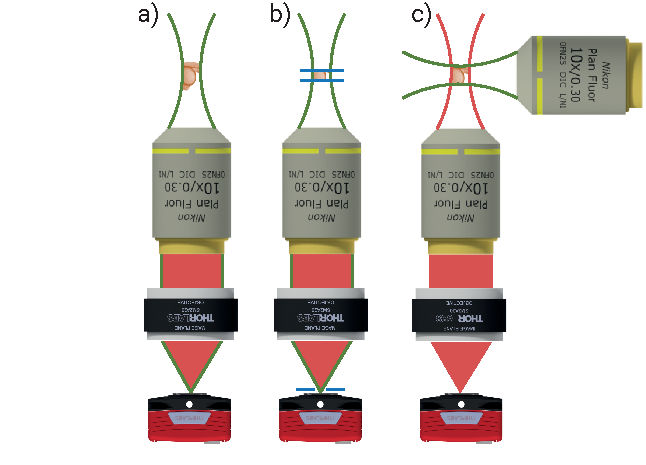
\includegraphics{./epi_con_lsfm}
%     \caption{}
%     \label{fig:epi_con_lsfm}
% \end{figure}

\begin{figure}
	\centering
        %\hspace{0.07\textwidth}
    \begin{subfigure}[t]{0.3\textwidth}
        \centering
        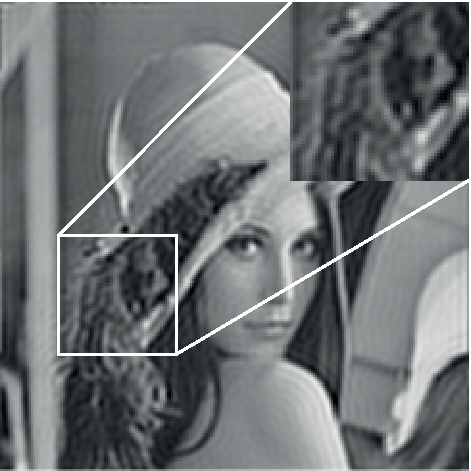
\includegraphics{epi_con_lsfm/widefield}
        \caption{Widefield imaging, epi-fluorescence; without \glslink{optical sectioning}{optical~sectioning}}\label{fig:epi_con_lsfm/widefield}
    \end{subfigure}
    \hfill%\hspace{0.01\textwidth}
    \begin{subfigure}[t]{0.3\textwidth}
        \centering
        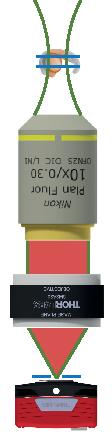
\includegraphics{epi_con_lsfm/confocal}
        \caption{Confocal imaging using a pin-hole at the imaging plane; epi-fluorescence, \glslink{optical sectioning}{optical~sectioning}}\label{fig:epi_con_lsfm/confocal}
    \end{subfigure}
        \hfill%\hspace{0.01\textwidth}
    \begin{subfigure}[t]{0.34\textwidth}
        \centering
        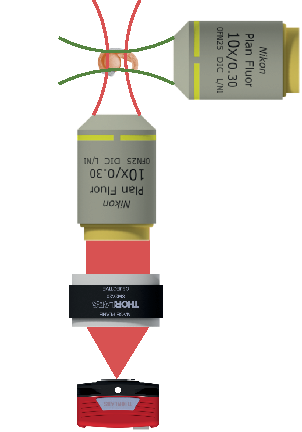
\includegraphics{epi_con_lsfm/spim}
        \caption{Widefield imaging with orthogonal illumination using a \gls{light-sheet}; \glslink{optical sectioning}{optical~sectioning}}\label{fig:epi_con_lsfm/spim}
    \end{subfigure}
    % \hspace{0.01\textwidth}
    %\hspace{0.07\textwidth}
    \caption[Comparison of \gls{wide-field}, \gls{confocal} and \gls{light-sheet} microscopy imaging modalities]
    {\Gls{light-sheet} microscopy (\subref{fig:epi_con_lsfm/spim}) combines the fast \gls{wide-field} imaging capabilities of epi-fluorescence microscopy (\subref{fig:epi_con_lsfm/widefield}) with the optical sectioning capabilities of \glslink{confocal microscope}{confocal microscopy} (\subref{fig:epi_con_lsfm/confocal}) which uses a narrow pinhole (blue) in a conjugate image plane to reject out-of-focus signal.
    }\label{fig:epi_con_lsfm}
\end{figure}


%High quality LSFM is dependent on how well the illumination is generated.
%Huisken et al seminally used Gaussian laser emissions for the generation of their light sheets.
%Gaussian beams have a distinct trade-off when used in LSFM applications in that the thinner the light sheet designed the narrower the field of view; this can be seen in equation \eqref{eq:Gaussian}, as $x$ increases or decreases (a movement away from the focus of the beam) the wider the beam gets.

%The Rayleigh length (or confocal parameter) in equation \eqref{eq:Rayleigh} is a metric for the distance over which a Gaussian beam still propagates as if it were parallel (neither converging nor diverging), for LSFM this is the distance over which it can be assumed the light sheet is of homogeneous thickness.

%Equation
%From equation \eqref{eq:Lorrentzian} g can be seen as having a dependence on the spot size or


% \section{Generating Light Sheets}
%
% \begin{itemize}
% 	\item[\checked] Optically  %\tick
% 	\item[\checked] Virtually
% 	\item[\checked] Volumetric Imaging
% \end{itemize}	%Lightfield is instant 3D

\subsection{Light-sheet generation}

High quality \gls{LSFM} is dependent on how well the illumination is generated, illumination can be generated all optically or using scanning techniques (digitally).

\subsection{Optical \gls{light-sheet} generation}
%TODO Etendue calculations


Huisken~\emph{et~al.} were seminal in their usage of Gaussian \gls{Laser} emissions for the generation of their light sheets.
\gls{Gaussian beam}s, however, have a distinct trade-off when used in LSFM applications, in that the thinner the light sheet the narrower the usable field of view.

Equations~\eqref{eq:GuasianBeam} to~\eqref{eq:Rayleigh} are the Gaussian beam approximation, which describes the propogation of a coherent Gaussian beam in free space.
The \gls{FWHM} (\(\sqrt{2\ln(2)}w(z)\)) %\mynote[inline]{check maths}
increases as a \gls{Lorentzian} (Equation~\eqref{eq:Lorrentzian}) when a distance \(z\) away from the focal plane depicted in \figurename~\ref{fig:GuasianBeam}.
The rate at which this occurs is dependent on the \gls{Rayleigh length} (\gls{z_R}) in Equation~\eqref{eq:Rayleigh} which quantifies the trade-off.
The confocal parameter (\(\gls{b}=2z_R\)) is a metric used to characterise the distance, centered on the beam waist, over which the Gaussian beam be approximately treated as a collimated beam (neither converging nor diverging).
% for the distance over which a Gaussian beam propagates as if it were parallel (neither converging nor diverging).
For \gls{LSFM} this is the distance over which the \gls{light-sheet} can be assumed to be of homogeneous thickness.

Huisken~\emph{et~al.} also pioneered the use of a cylindrical lens to focus the \gls{Gaussian beam} along one dimensional into a Gaussian \gls{light-sheet}.
For \gls{LSFM}, the Gaussian intensity profile of a \gls{Gaussian beam} requires that the excitation beam is over expanded and later cropped by an aperture to create a homogeneous illumination profile.
% The Gaussian nature of a beam's intensity for \gls{LSFM} requires that the excitation beam is over expanded and later cropped by an aperture to create homogeneous illumination.
The procedure is optically lossy, but not a problem in practise as, \gls{Laser} intensity is typically in surplus in \gls{wide-field} fluorescence microscopy techniques.
A typical good fluorescent sample may require \SI{2(1)}{\milli\watt} and a typical
% in comparison to a low end
diode \gls{Laser} emits
% ing
\SI{100}{\milli\watt}+.

%Huisken's SPIM had two distinct parts.
%The illumination path, which included a laser source beam expander to control the field of view of the light sheet and a  cylindrical lens to focus the beam into a thin sheet of light (Fig %FIGURE
%); and the detection path, which was similar to a standard widefield microscope including an objective lens, a tube lens and a camera.

\begin{figure}
    \centering
    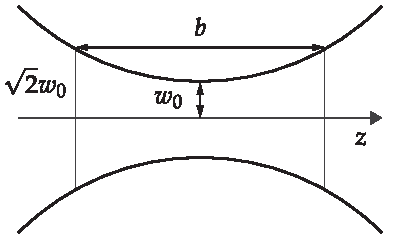
\includegraphics{./GuasianBeam}
    \caption[Schematic of the propagation of a Gaussian beam]{Schematic of the propagation of a Gaussian beam.
    The beam is assumed to be collimated (par-axial) within the length \gls{b} (the confocal parameter) for a given spot size \gls{w_0}.
    The spreading of the beam obeys a Lorentzian hyperbole as in Equation~\eqref{eq:Lorrentzian}}\label{fig:GuasianBeam}
\end{figure}

\begin{align}
	I(r,z)    & = {I_0} {\left(\frac{w_0}{w{(z)}}\right)}^2 {e^{\frac{-2r^2}{w{(z)}^2}}\label{eq:GuasianBeam}} \\
	w(z) & = \gls{w_0} \sqrt{1+\frac{z}{z_R}} \label{eq:Lorrentzian}                                                   \\
	z_R       & = \frac{\pi w^2}{\lambda} \label{eq:Rayleigh}
\end{align}

Where \gls{z_R} is the \gls{Rayleigh length}; \gls{w_0} is the spot of size of the beam and \gls{lambda} is the wavelength of light.

% Introduce Gaussian beam
% In cylindrical lens case laser light needs to be over expanded and cut to ensure a FOV homo

\subsection{Digital \gls{light-sheet} generation}

%Cylindrical lenses are bad because the sheet is highly coherent causing interference and more shadowing.
%A light-sheet crafted just using a cylindrical lens comes with it's own issues.
%Keller et al addressed
Keller~\emph{et~al.}~\cite{keller_quantitative_2008} proposed sweeping a narrow collimated \gls{Laser} beam through the sample to create a \gls{virtual light-sheet}.
This was achieved by oscillating galvanometric mirrors at \SI{}{\kilo\hertz} frequencies, well over the Nyquist limit in comparison to the imaging acquisition rate of \SI{<100}{\hertz}~\cite{keller_quantitative_2008}.
To ensure a homogeneous illumination and distributed photon dosage a \gls{telecentric} f\(\theta \) lens was used to convert beam angle optically from the scanning mirrors in to a linear position~\footnote{A practice borrowed from \gls{Laser} scanning microscopy.}.

Using \gls{DSLM} instead of a cylindrical lens based system offers some key advantages.
Firstly, as the beam is scanned rather than optically stretched there can be no optical interference of coherent photons between neighbouring regions in the sample, this reduces speckles and shadows.
Secondly, illumination intensity can be modulated such that structure can be superimposed on the sample giving the potential for \gls{super-resolution} image improvement using \gls{SIM} as in Section~\ref{sec:SIM_theory}.
This resolution improvement has so far solely been experimentally demonstrated in the direction of the the scanning due to geometrical constraints~\cite{chen_lattice_2014}.

\subsection{Volumetric imaging}

The most valuable aspect of \gls{LSFM} is its capability to perform fast volumetric imaging.
Huisken's original \gls{SPIM} required the samples to be scanned mechanically through the static light sheet, potentially perturbing the sample, depending on the speed of the scanning.
\gls{DSLM} improves upon the static \gls{light-sheet} by using a second galvanometric mirror to move the \gls{light-sheet} relative to the static sample, the detection objective is then mounted on a high speed and precision axial translator and tuned to follow the \gls{light-sheet}.
Ideally, piezoelectric actuators are used as their settling times are on the order of milliseconds which provides the speed and accuracy needed to match \SI{100}{\hertz} imaging cameras.

\subsubsection{Remote focusing}

With \gls{DSLM}, instead of the stage motion causing possible disturbance of the specimen, there is a risk that motion of the objective lens near to the specimen causes turbulence.
This mechanical motion can be eliminated by placing an
% This was matched optically through the use of an electrically
\gls{ETL} in the detection path.
In Fahrbach~\emph{et~al.}~\cite{fahrbachRapid3DLightsheet2013} system, the \gls{ETL} was used to shift the \gls{working distance} of the detection objective to match the scanning \gls{light-sheet}.
%As such a new method was developed to achieve this optically, by using an electrically tunable lens to adjust the working distance of the detection objective.
The technique suffers from fluorescent signal losses in the further four lenses and two mirror surfaces required (\SI{\sim80}{\%} signal retrieved).
\footnote{The mirrors are used to ensure the \gls{ETL} is horizontal to gravity as further aberrations occur if the tunable surface is not entirely flat.
Two mirrors from the tunable light sheet could be removed by using mechanically deforming tunable lenses instead of electro wetting tunable lenses.}
The technique is also prone to spherical aberration, and is a more involved method as the system requires a non-linear calibration.
Huisken~\emph{et~al.} showed, using a contrast grid, that image quality and aberrations are negligibility affected;
and they demonstrated
% then proceeded to produced
\SI{100}{\hertz} volumetric imaging, though on small volumes~\cite{fahrbachRapid3DLightsheet2013}.
Disaspro~\emph{et~al.} improved upon using \gls{ETL}s by optically relaying a virtual image of the sample and using a secondary microscope, with an actuated objective; the result was inertia-free imaging with fewer optics and fewer \gls{ETL}-induced aberrations~\cite{duocastellaFastInertiaFreeVolumetric2017c}.

% \subsubsection{Remote focusing} %TODO could be somewhere else

%There are three ways in which to realise the full three dimensional SPIM.
% The simplest way is to move the sample through the light sheet as is done in Oblique Plane Imaging.
% The second method involves scanning the light sheet through \textit{z} which is potentially faster; the issue which then arises is that the light sheet moves out of the focal plane of the detection objective.
% The focal plane can be moved onto the light sheet by moving the excitation objective, however this method (like the first method) causes perturbations to the sample.

%Tunable lens technology is exceptionally young compared to the history of glass optics and so its image aberration correction is not as well implemented.
%To that end critics of this technique suggest that a tunable lens in the detection arm will inherently introduce noticeable image degradation.

%Image of four configurations with details.
\section{Objective arrangements}
\subsection{Single view imaging}
%To ensure compatibility of Light sheet microscopes with biological mounting arranging.
\Gls{light-sheet} microscopes are distinctive in that two objective lenses are used orthogonally.
This causes the technique to be incompatible with most standard \gls{epi-fluorescence} biological mounting practices.
Efforts have been made to make \gls{light-sheet} imaging more compatible through novel objective arrangements as well as new sample mounting approaches.

\subsubsection{Horizontal orientation}

% \begin{itemize}
% 	\item[\checked]  Flat (openSPIM) open-SPIN diy-SPIM
% 				\item[\checked] MuVIEW\cite{swoger_multi-view_2007}%CITE"3060
% 	\item[\checked] Vert
% 	\item[\checked] V (diSPIM)
% 	\item[\checked] 60/30		Lattice Light Sheet and Objective Compatibility (Short section)
% 	\item[] Multi VIEW
% \end{itemize}

%and the excitation objective illuminating through a clear window in the chamber.
Huisken~\emph{et~al.}, for instance, mounted two objectives in a horizontal configuration; a detection objective built into a sample chamber and illuminated using a \gls{light-sheet} through a clear window~\cite{huisken_optical_2004}.
This configuration was chosen so that a sample could be lowered into the system and, crucially, rotated without gravity causing registration errors when reconstructing the volume \glslink{tomography}{tomographically}.%, see \figurename~\ref{fig:depth/ispim}.
Rotational volumetric imaging also minimises shadows and improves image quality lost to scattering especially in thick \SI{>500}{\micro\meter} samples as in \figurename~\ref{fig:depth/spin_spim}.
Mounting a sample from below and rotating produces the same result but requires a more sophisticated chamber design to contain the sample medium.
A horizontal geometry is important for imaging plant biology, as the objectives do not inhibit the plant's natural tendency to grow upright~\cite{wangenheimRulesSelfOrganizingProperties2016a}. %TODO CITE Stelzer
%Long working distance detection objectives have also been considered but the the lowered NA and

\subsubsection{Vertical orientation}

An alternative to the horizontal configuration is mounting the detection objective vertically above the sample, and then illuminating the sample from the side.
A vertical orientation is attractive as it can be compatible with commercial optical microscopes as well the chamber not requiring an inbuilt detection objective~\cite{schlegel-zawadzkaFluorescenceImagingSpectroscopy1997,wuSpatiallyIsotropicFourdimensional2013}.
Both of these techniques can allow for an additional illumination objective with counter-propagating illumination.
By offsetting the foci of the illumination objectives along the axis of propagation an overall more homogenous illumination profile can be created, with reduced shadows.

\subsubsection{\SI{45}{\degree} orientation}

Shroff~\emph{et~al.} then pioneered use of two objectives in a `V' configuration above the sample through \gls{iSPIM}.
With carefully chosen objectives, whereby the sum of the opening angles of both objectives does not exceed \SI{180}{\degree},
samples prepared with standard mounting procedures may be imaged in a petri-dish or glass~slides~\cite{kumarDualViewPlaneIllumination2014}.
%Other group then did the 45 degree inverted iSPIM.
%Shroff's diSPIM~\cite{kumar_dual-view_2014} then drastically improved axial resolution by imaging through both arms of the microscope.
%In doing so the axial resolution not collected through one arm is directly observed in the other.

%CITE 30 chick embryos

% \begin{figure}
% 	\centering
% 	\includegraphics[width=\columnwidth]{spim_optimal_imaging.png}
% 	\caption{
% 	(a): The simple SPIM field of view – only a quarter of a sample has optimum illumination (green) and excitation (red).
% 	(b): by rotating a sample field of view can be quadrupled but at a cost in acquisition time.
% 	(c): By adding extra excitation and detection path the entire sample can be imaged without a rotation.
% 	(d): by making optical paths of a LSFM dual purpose a quadrant of a sample can be imaged from two orthogonal perspective and with correct image fusion achieve isotropic resolution.
% 	tod}
% 	\label{spim_optimal_imaging}
% \end{figure}
%

\begin{figure}
	\centering
    \begin{subfigure}[t]{0.4\textwidth}
        \centering
        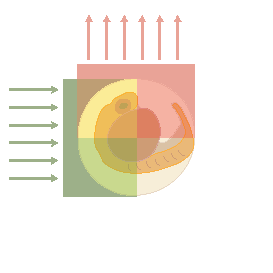
\includegraphics{depth/ispim}
        \caption{Single detection, single illumination~\cite{wuInvertedSelectivePlane2011a}}\label{fig:depth/ispim}
    \end{subfigure}
    \hspace{0.07\textwidth}
    \begin{subfigure}[t]{0.4\textwidth}
        \centering
        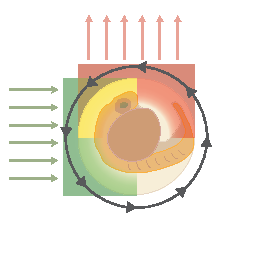
\includegraphics{depth/spin_spim}
        \caption{Single detection, single illumination, with sample rotation~\cite{huisken_optical_2004}}\label{fig:depth/spin_spim}
    \end{subfigure}
    \begin{subfigure}[t]{0.4\textwidth}
        \centering
        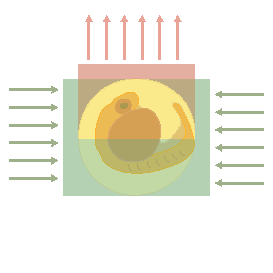
\includegraphics{depth/dual_illumination}
        \caption{Single detection, dual illumination~}\label{fig:depth/dual_illumination}
    \end{subfigure}\hspace{0.07\textwidth}
    \begin{subfigure}[t]{0.4\textwidth}
        \centering
        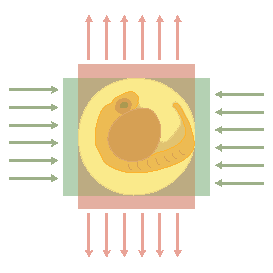
\includegraphics{depth/multiview}
        \caption{Dual detection, dual illumination~\cite{krzicMultiviewLightsheetMicroscope2012}}\label{fig:depth/multiview}
    \end{subfigure}
    \begin{subfigure}[t]{0.4\textwidth}
        \centering
        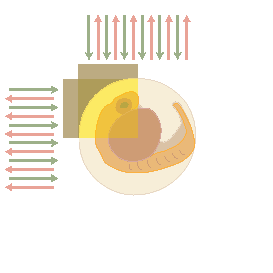
\includegraphics{depth/di_spim}
        \caption{Single detection, single illumination, with alternate illumination and detection~\cite{kumar_dual-view_2014}}\label{fig:depth/di_spim}
    \end{subfigure}\hspace{0.07\textwidth}
    \begin{subfigure}[t]{0.4\textwidth}
        \centering
        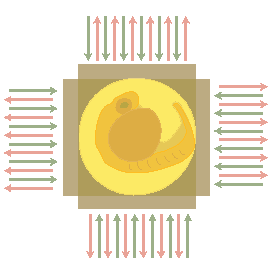
\includegraphics{depth/muvi}
        \caption{Dual detection, dual illumination, with alternate illumination and detection}\label{fig:depth/muvi}
    \end{subfigure}
        \caption[Schematic of objective lens arrangements for optical \gls{light-sheet} imaging]{Schematic of objective lens arrangements for optical \gls{light-sheet} imaging.
        p.t.o}
\end{figure}
\begin{figure}
\ContinuedFloat\caption[]{
        (\subref{fig:depth/ispim}) and (\subref{fig:depth/spin_spim}) both use a single objective lens for imaging and illumination, with (\subref{fig:depth/spin_spim}) rotating the sample so that optimal imaging is not limit to the \emph{optical quarter} (yellow).
        (\subref{fig:depth/dual_illumination}) adds an additional illumination objective to mitigate illumination light lost through sample penetration.
        (\subref{fig:depth/multiview}) adds a further imaging objective lens to mitigate detected light being lost to sample penetration; the images of each detecting objective are later computationally fused.
        (\subref{fig:depth/di_spim}) uses a pair of illumination and detection lenses to enhance the resolution (deeper yellow) in the \emph{optimal quarter}, by fusing the data from each objective alternately.
        (\subref{fig:depth/muvi}) repeats the imaging and illumination alternation approach from (\subref{fig:depth/di_spim}) but does so in four objectives instead of two.
        \textbf{Image acquisition speeds}:
        % (\subref{fig:depth/spin_spim}) is the same as (\subref{fig:depth/ispim}).
        (\subref{fig:depth/spin_spim}), (\subref{fig:depth/dual_illumination}) and (\subref{fig:depth/multiview}) are the same speed as (\subref{fig:depth/ispim}) but (\subref{fig:depth/multiview}) requires a computational reconstruction in post-processing.
        (\subref{fig:depth/di_spim}) is half the speed of (\subref{fig:depth/ispim}) and (\subref{fig:depth/muvi}) is a quarter the speed of (\subref{fig:depth/ispim}), both requiring extensive post-processing computation.
      }\label{fig:spim_optimal_imaging}
\end{figure}

\subsubsection{Optimal orientation}

In an attempt to maximise sample accessibility and numerical aperture, Betzig~\emph{et~al.}~\cite{chenLatticeLightSheetMicroscopy2014} commissioned a high \gls{NA}~(\SI{0.6}{}) custom excitation objective to fit with the high \gls{NA}~(\SI{1.1}{})~\gls{LWD} detection objective (Nikon CFI75).
A custom excitation objective was needed as high~\gls{NA} objectives are physically large with short \gls{working distance}s.
In mounting the orthogonal pair at an angle such that they were planar so a flat surface, Betzig~\emph{et~al.} maximised detection and excitation \gls{NA} whilst minimising sample mounting impedance.

% Theer~\emph{et.~al.} \cite{theerPSPIMHighNA2016}
% created the most unhindered sample mounting conditions realistically feasible using two objectives.
% Tricks to circumvent objectives interfering with sample mounting are needed as high~\gls{NA} objectives are physically large.
%Numerical aperture depends on the $\sin$ of the collecting angle of light , intuitively this requires that the detecting objective to awkward in non-epifluorescence orientations. \mynote{reword}
%Moreover, the desire for high resolution images can cause spacial incompatibility between both objectives.
% Moreover, high \gls{NA} objectives typically have short \gls{working distance}s and require both objectives to be close, and likely cause spacial incompatibilities even with the narrowest excitation objectives.
% See figure~\ref{fig:objectivecompatibility} for a detailed comparison.
%
% \begin{figure}
% 	\includegraphics[width=\columnwidth]{objectivecompatibility}
% 	\label{fig:objectivecompatibility}
% 	\caption{}
% \end{figure}

%Gaussian light sheet systems do not typically require such large NA excitation objectives meaning there are standard excitation objectives available.
%High NA objectives tend to have limited working distance and, in the orthogonal arrangements required for LSFM, have to be positioned very close to each other.

%suitably narrow such that flat substrates could be imaged.
%lattice light sheet style custom excitation.

%Gaussian beams don't need high NA excitation optics
%Large NA detection objectives have large collecting angles so a long working distance objective in desirable.


%subsection{MultiView}
\subsection{Multi-view}%\cite{swoger_multi-view_2007}

Shroff~\emph{et~al.} introduced alternate imaging between each objective of the \gls{iSPIM} in the form of the \gls{diSPIM}~\cite{kumar_dual-view_2014}, depicted in \figurename~\ref{fig:depth/di_spim}%TODO Repeating myself
\footnote{This system is now a commercial \gls{light-sheet} solution provided by ASI.}.
Axial resolution that would otherwise be lost to thick \gls{light-sheet}s is recovered by switching the imaging and detection arms.
The two data sets captured by each camera are fused in post processing to provide near isotropic three dimensional resolution.
%\subsubsection{DualView}
%Shroff~\emph{et~al} not only pioneered the inverted SPIM (iSPIM) concept but also introduced alternately imaging between each objective in the form of diSPIM~\cite{kumar_dual-view_2014}. %TODO Repeating myself
%Axial resolution that would otherwise be lost to thick light sheets is recovered by switching the imaging and detection arms.
%The two data sets captured by each camera are fused in post processing.
%subsection{MuVU}
Where \gls{LSFM} provides the most improvement over other techniques, such as in large, thick biological samples;
%Where LSFM provides most improvement over other techniques
scattering induced image degradation then becomes significant, both for excitation and emission light.
For imaging in thick samples using orthogonal detection and excitation there does exist an
% Though\gls{diSPIM} however does not address inherent issues of scattering in thick samples, there is an
\emph{optimal quarter} (see \figurename~\ref{fig:spim_optimal_imaging}) wherein excitation and emission photons are the least scattered.

Krzic~\emph{et~al.} used the horizontal orientation of Huisken's \gls{SPIM}, in \gls{MuVi-SPIM} (\figurename~\ref{fig:depth/multiview}) where two excitation and two detection objectives were packed around a hanging sample~\cite{krzicMultiviewLightsheetMicroscope2012}.
%cite objectives (Krzic et al. 2012)
\gls{MuVi-SPIM} is able to image all regions of the sample. %but it cannot dodge scattering limitations homogeneously.
%\subsection{Tomography}
To minimise gross sample scattering, sample rotation is necessary.
Acquiring volumes via rotational \glslink{tomography}{tomographically} raises further unique issues such as volume registration, rotational synchronisation and longer acquisition times.
% For large samples two objectives in Huiksen's original SPIM provide a cost effective robust volumetric imaging solution; with projects like the OpenSPIM have received significant acceptance and community attention.

\section{Single objective \gls{light-sheet} microscopy}

% \begin{itemize}
% 	\item[\checked] Axial Plane \cite{li_axial_2014}
% 	\item[\checked] Oblique Plane \cite{dunsby_optically_2008}
% 	\item[\checked] Fibre SPIM \cite{ploschner_multimode_2015}
% 	\item[\checked] Mirrored Cuvette,
% 	\item[\checked] Confocal adaptor
% \end{itemize}

Prior to refinements in objective positioning from the last section, Dunsby~\emph{et~al.} conceptualised a system for single objective \gls{light-sheet} microscopy.
\footnote{The advent of such systems could provide a plug-and-play \gls{light-sheet} experience on commercial microscope frames.}
Dunsby~\emph{et~al.} proposed illuminating the sample using an objective with a large aperture whereby the \gls{light-sheet} would illuminate at an oblique angle to the optical axis, the detected signal is then retrieved using the same objective~\cite{dunsby_optically_2008}.
Optically, the sample is conjugated to a virtual position where a pair of objectives (excitation and detection) analyse the virtual sample in a conventional \gls{light-sheet} manner, which is shown in \figurename~\ref{fig:single_objectives/opm}.
The technique suffers in that only half the imaging \gls{NA} may be collected.
% The technique suffers from optical technology, only when using a high \gls{NA} objective can the system fully capture detection perpendicular to excitation.
\gls{OPM} is an involved technique as it requires that a \gls{light-sheet} microscope is constructed, behind an optical relay system, relaying the virtual image from a standard microscope body.

\gls{SCAPE} uses the same principle as \gls{OPM} but attempts to greatly reduce the optics and labour required.
Hillman~\emph{et~al.} do so by using a single polygonal mirror in the infinity space of the detection objection to redirect excitation and emission light~\cite{bouchardSweptConfocallyalignedPlanar2015}, see \figurename~\ref{fig:single_objectives/scape}.
The polygonal mirror then rotates to sweep the light-sheet and detecting focal plane through the sample.

Virtual sample manipulation is alluring as virtual manipulations can be performed that in are impossible physically.
Zhang~\emph{et~al.}~\cite{li_axial_2014} created a virtual sample using a similar relay system to Dunsby~\emph{et~al.}, but crucially they positioned an atomically flat mirror which rotated their virtual sample by \SI{90}{\degree}, shown in \figurename~\ref{fig:single_objectives/atomic_mirror}.
In doing so, the real sample could be illuminated along the optical axis and the mirrored virtual projection was imaged directly onto a camera. % using a standard wide field configuration.

Using small mirrors near the sample is another viable, though more restrictive, approach to single objective \gls{LSFM}.
Galland~\emph{et~al.} fabricated micro-wells with \SI{45}{\degree} micro-mirrors~\cite{galland_3d_2015}, converting any commercial scanning microscope into a \gls{light-sheet} microscope
\footnote{Leica produce a similar solution in the form of an objective adapter which holds two mirrored surfaces near the sample creating a similar effect.}.
Both techniques limit the size of the sample and their sectioning capability heavily depends on the quality of the mirrors used.

Ploschneret~\emph{et~al.} minimised the size of the second excitation objective rather than remove it by substituting the it for a multimode fibre~\cite{ploschner_multimode_2015}.
% This provided more access to samples %but they were able to embed
% ot only could they provide more access to their samples, but they could also embed their excitation source into their imaging chamber.
By assuming that a multi-mode fibre operates deterministically on an input light source, Ploschneret~\emph{et~al.} were able to homogenise the illumination output of the fibre using an \gls{SLM}.
They then demonstrated the \gls{exotic beam} profiles using the same \gls{SLM}.

% \clearpage
\begin{figure}
  \centering
  \begin{subfigure}[t]{\textwidth}
    \centering
    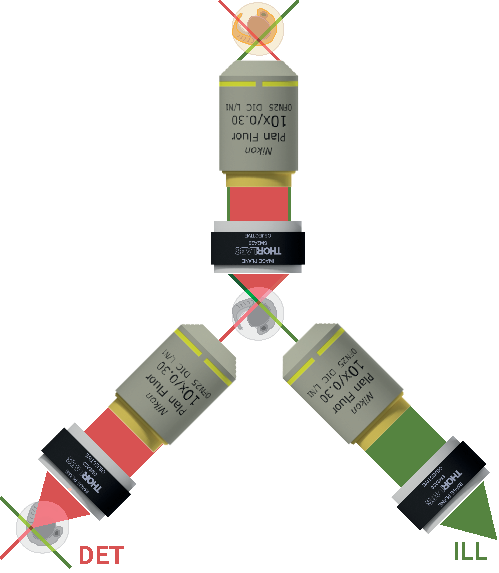
\includegraphics{single_objectives/opm}
    \caption{\gls{OPM}~\cite{dunsby_optically_2008}}\label{fig:single_objectives/opm}
  \end{subfigure}
  \begin{subfigure}[t]{0.475\textwidth}
    \centering
    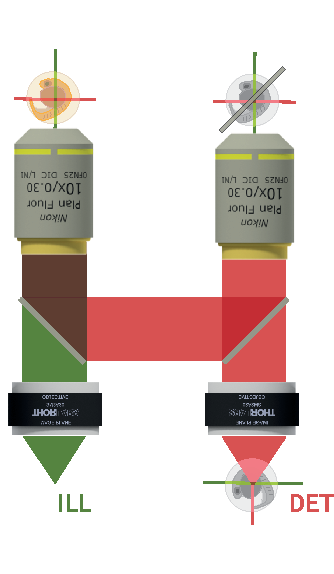
\includegraphics{single_objectives/atomic_mirror}
    \caption{Atomically flat mirror to rotate virtual image~\cite{li_axial_2014}}\label{fig:single_objectives/atomic_mirror}
  \end{subfigure}
  \begin{subfigure}[t]{0.5\textwidth}
    \centering
    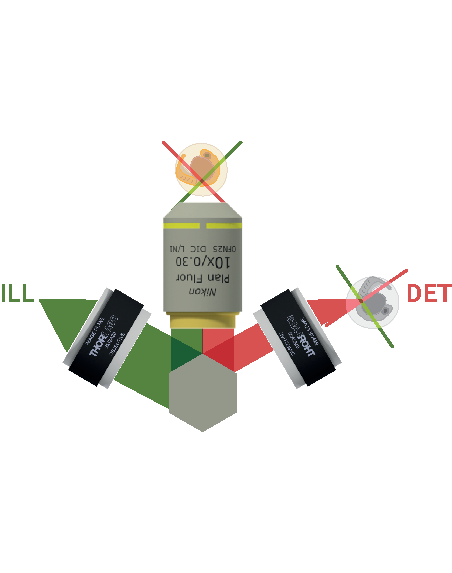
\includegraphics{single_objectives/scape}
    \caption{\gls{SCAPE}~\cite{bouchardSweptConfocallyalignedPlanar2015}}\label{fig:single_objectives/scape}
  \end{subfigure}
  % % \includegraphics{/path/to/figure}
  \caption[]{
  % % Input sheet illumination is at ILL and the detection or imaging plane is at DET.~Samples in orange are real objects, samples in grey are virtual objects.
  p.t.o}
  \end{figure}
  \begin{figure}
    \ContinuedFloat\caption[Depiction of three choice methods for light-sheet microscopy using a single objective lens at sample]{
  Depiction of three choice methods for light-sheet microscopy using a single objective lens at sample.
  All the methods presented are therefore compatible with standard mounting techniques and standard microscope frames.
  In (a), a light-sheet is introduced into the sample at, and imaged at, an oblique angle to the primary objective lens.
  The sample image is relayed and it's virtual image is then relayed by a separate imaging path onto a detector.
  The system in (b) relays the image of the sample onto an atomically flat mirror, which rotates the virtual image when it then relayed the detector.
  For (c), a polygonal mirror is used to illuminate and image the sample at oblique angles, similar to \gls{OPM}.}\label{fig:single_objectives}
\end{figure}
% \clearpage
%TODO cite scape

%subsection{Axial Plane}~\cite{li_axial_2014}
%subsection{Oblique Plane}~\cite{dunsby_optically_2008}
%subsection{Fibre SPIM}~\cite{ploschner_multimode_2015}

%Optical fibre transforms input light, can comepnsate and produce light sheets, bessel light sheets and lattice etc.
%Demonstrated in 0.25 NA fibre.
%Could use soft glass fibre to prove concept further.

%subsection{Confocal adaptor}

% High NA objectives require short working distances and large apetures
% An asymmetric pair
% an NA of 0.3 is needed to create a micron thick miaskla kzas
% Gaussian beam illumination requires low NA excitation and so assymetric pairs are ideal with a high NA detection being then possible (with a loss of axial resolution)
% Bessel illumination however requires high NA to construct the thin buy extended sheets and so are commcercially infeasible.
%Betzig et al. notabley used a custom excitation objective.
% Biological samples should be given room.

% Hence the ‘vertical at 90o’ approach can very attractive even if it cannot boast high NA excitation.
%Another limitation arises from geometrical compatibility of the objectives i.e. their opening angles cannot exceed 90o and the front lens radius of one objective should not exceed the working distance of the other objective.

%High NA detection and low NA excitation leads to high lateral resolution and low axial resolution.

\section{Illumination}

%\begin{itemize}
%	\item Variable Gaussian $\box$
%	\item Bessel\cite{gao_3d_2014}
%	\item Lattice light sheet.\cite{chen_lattice_2014}
%	\item Airy Beam $\box$
%	\item Multi-photon \checkmark~\cite{truong_deep_2011}
				%Comparison of Cost and Complexity?
%\end{itemize}

Novel illumination techniques have been proposed in a bid to circumvent the ubiquitous Gaussian beam extension to sheet thickness trade-off and minimising shadowing artefacts.

\subsection{Gaussian techniques}

Santi~\emph{et~al.} proposed using a Gaussian sheet with a narrow \gls{FOV}, scanning the sample and stitching the result~\cite{santiThinsheetLaserImaging2009}.
% The most intuitive approach is accepting the loss of \gls{FOV} produced by Gaussian illumination and moving the focus of this strip of high axial resolution light to different parts of the sample.
A final image can then be fused to achieve maximum axial resolution though with a direct cost for time of acquisition and photobleaching versus axial resolution, with an exceptionally high \gls{NA} light sheet tending to becoming as slow and damaging as a confocal system.
Chmielewski~\emph{et al.} expanded on this concept by using tuneable lenses to dynamically adjust the extent and width of their \gls{light-sheet}s~\cite{chmielewskiFastImagingLive2015}.

% \mynote{CITE Variable light-sheet.}
Fu~\emph{et~al.} proposed the superposition of multiple thin and focally-offset Gaussian \gls{light-sheet}s to create a tiling effect without the loss of temporal resolution~\cite{fu_imaging_2016}.
%The technique of tiled light-sheets was proposed recently whereby multiple thin Gaussian light-sheets are superimposed and focally offset to create a similar tiling effect without the temporal loss \cite{fu_imaging_2016}.
The tiling effect was produced by using an \gls{SLM} whose hologram had multiple lens-like (quadratic) phase patterns superimposed.
The technique suffers from the additional photo-dosage imparted from the undesirable lobes of the Gaussian beam, moreover these low axial-resolution sections also contribute fluorescent background reducing the net \gls{SNR} of the system.

In \gls{mSPIM} Huisken~\emph{et~al.} added an additional scanning mirror to control the emission angle of the \gls{light-sheet}.
By dithering this mirror slightly during an acquisition shadowing artefacts were markedly reduced~\cite{huiskenEvenFluorescenceExcitation2007}, see \figurename~\ref{fig:scatteringandshadowing}.

\subsection{Exotic beams}

Several \gls{exotic beam}s exist which have been used to avoid the
% and whose properties do not subscribe to
classical \gls{Gaussian beam} limitations, particular the trade-off between thinner and useful extent of the light-sheet, along the illumination axis.
%Airy beams, for instance, are non-diffracting, self healing beams.
% and I don't know anything about them over that Nikon use them?
\subsection{Bessel beams}

\gls{Bessel beam}s are non-diffracting and ``self-healing'' non-diffracting beams, they produce thin long beams which reconstruct behind occlusions (see \figurename~\ref{fig:exotic_beams_cartoon_exotic}), making them very desirable for light-sheet applications.
They can be optically constructed from either an \gls{axicon} lens or a amplitude mask with a annular ring opening, the latter being inexpensive but the most optically lossy.
Unlike Gaussian beams the extension and thickness of a theoretical \gls{Bessel beam} can be entirely decoupled, in practice a \gls{Bessel beam}s only behave as such over short distances~~\cite{gao_3d_2014} of up to \SI{\sim30}{\micro\meter}.
%\mynote[inline]{how short?}
% with the thickness being controlled by the outter-most radius and their extension
%Be beams both self heal,
\gls{Bessel beam}s, however, suffer from having multiple undesirable outer orders; the more ideal a \gls{Bessel beam} is, the closer the ratio of the energy of the central beam versus outer lobes is to \SI{1}{}.
As such, a singular scanned \gls{Bessel beam} causes a significant background signal as the additional lobes contribute as out-of-focus signal.
Betzig~\emph{et~al.} exploited these additional orders by constructing multiple \gls{Bessel beam}s in the scanning plane~\cite{chen_lattice_2014}.
The spacing of which was controlled by varying the periodicity of the
% Achieved by superimposing a
sinusoidal amplitude pattern (diffraction grating) on an annular amplitude mask (\gls{Bessel beam} mask).
In doing so, the undesirable orders constructively interfered to reinforce the zeroth orders of the parallel beams.
Finally, they tuned the periodicity \gls{lattice light-sheet} such that the outer orders above and below the scanning plane lay at the first minima in the detection \gls{PSF} reducing the net fluorescent axial background.

\subsubsection{Airy Beams}

\gls{Airy beam}s also self-heal similarly to \gls{Bessel beam}s but are more extended comparatively.
\gls{Airy beam}s are constructed using a \glslink{comatic aberration}{coma}-like (cubic) phase pattern and exhibit a characteristic beam curvature.
The curvature produces an asymmetric profile along the detection axis, which then needs to be \glslink{deconvolution}{deconvolved} in post-processing.
% Though they extend several fold further than \gls{Bessel beam}s,
% This is then required to be deconvolved in post processing.
Vettenburg~\emph{et~al.} demonstrated a similar axial resolution improvement as with \gls{Bessel beam}s, whilst achieving a \SI{\sim3}{} increase in \gls{FOV}~\cite{vettenburg_light-sheet_2014}.
%It logically follows to create a lattice of Airy beams, this
%\mynote[inline]{TODO cite.}
%Airy beams are generated with a phase distribution resembling coma aberrations.
%These beams are characterised by longer extent compared to typically achievable Bessel beams (e.g. extension of 160 µm versus 60 µm for a Bessel beam with similar diameter) (Vettenburg et al. 2014).
%However, the Airy beams exhibit a curvature similar to coma aberrations and unsymmetrical higher orders in the beam radial profile, creating a PSF with characteristic unsymmetrical elongation along the detection axis (Morris et al. 2009). These can be corrected by deconvolving a measured stack using software methods.
%This can produce better resolution images with larger field of view compared to similarly deconvolved images obtained using Gaussian and Bessel beams (Vettenburg et al. 2014).
%However, this superiority over Bessel beams has only been demonstrated in comparison with the most basic Bessel beam setup, which does not compensate for higher orders of the Bessel beam distribution

% \begin{figure}
% 	\centering
% 	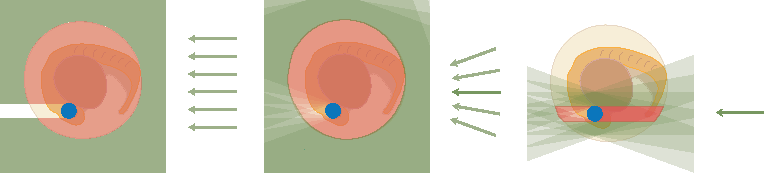
\includegraphics{exotic_beams_cartoon}
%     \caption{}
%     \label{fig:scatteringandshadowing}
% \end{figure}

\begin{figure}
	\centering
    \begin{subfigure}[t]{0.3\textwidth}
        \centering
        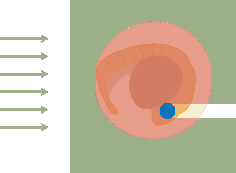
\includegraphics{exotic_beams_cartoon_para}
        \caption{Par-axial \gls{light-sheet} illumination}\label{fig:exotic_beams_cartoon_para}
    \end{subfigure}
    \hfill
    \begin{subfigure}[t]{0.3\textwidth}
        \centering
        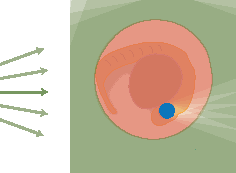
\includegraphics{exotic_beams_cartoon_mspim}
        \caption{\gls{mSPIM}, multi-directional \gls{light-sheet} illumination}\label{fig:exotic_beams_cartoon_mspim}
    \end{subfigure}
    \hfill
    \begin{subfigure}[t]{0.3\textwidth}
        \centering
        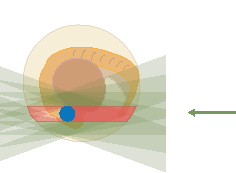
\includegraphics{exotic_beams_cartoon_exotic}
        \caption{Par-axial Bessel beam illumination.}\label{fig:exotic_beams_cartoon_exotic}
    \end{subfigure}
    \caption[Shadowing artefacts in light-sheet can be mitigated through different types of illumination]{
    Shadowing artefacts in light-sheet microscopy (\subref{fig:exotic_beams_cartoon_para}) can be mitigated through different types of illumination.
    (\subref{fig:exotic_beams_cartoon_mspim}) uses \gls{light-sheet}s from multiple directions to illuminate behind an occlusion.
    (\subref{fig:exotic_beams_cartoon_exotic}) uses Bessel sheets which have the property of self-healing behind occlusions; this happens as Bessel beams arise from constructive interference from angled plane waves.%, which then reach behind the occlusion.
    % from multiple directions to illuminate behind an occlusion.
    }\label{fig:scatteringandshadowing}
\end{figure}

\subsection{Thinner sheets}

% Attempts to quantum mechanically narrow Gaussian Light sheets include using \gls{STED} and \gls{2P} excitation.
By exploiting the quantum mechanical nature of \gls{fluorophore}s, methods for further improving sheet thickness have included using \gls{STED} and \gls{2P} excitation.
Using an addition \gls{Laser} to deplete the excitation sheet (using \gls{STED}) out of plane fluorescence can narrow a Gaussian light sheet to \SI{<1}{\micro\meter}~\cite{friedrich_sted-spim:_2011}.
\gls{2P} \gls{light-sheet} microscopy uses the the narrowing effect of \gls{2P} (Section~\ref{sec:2p}) excitation to create a narrow excitation sheet.

\section{Summary}

Light-sheet microscopy can be used to acquire fast volumetric imaging data.
Typically this achieved with two orthogonal objectives, each for excitation and detection.
Having multiple objectives near a biological sample does however impede traditional mounting strategies.
Classical light-sheets have a dependancy between their \gls{FOV} and axial thickness, these constraints can be overcome with exotic illumination modalities.

The techniques and methods presented here for generating \gls{light-sheet}s and detecting the resultant fluorescence, in thick biological samples, will be used in the following chapter to inform the design of a 3D-particle tracking \gls{light-sheet} microscope.
% \vspace{0.5\textheight}
% \section{Extended depth of field}

% \section{Scape}
% Hyper spectral spim
% Axially swept light-sheet geometries.

%% Some final comments
